% \begin{filecontents}{\jobname.bib}
% @book{Dumke2001,
%     Author = {Dumke},
%     Publisher = {Vieweg},
%     Title = {Software-Engineering},
%     Year = {2001},
%     ISBN = {3-528-25355-X}}
% @book{Balzert1998,
%     Author = {BALZERT, H.},
%     Publisher = {Spektrum Akademischer Verlag},
%     Title = {Lehrbuch der Software-Technik, Band 2: Software-Management, Software-Qualit"atssicherung},
%     Year = {2001},
%     ADDRESS = {Heidelberg; Berlin; Oxford},
%     ISBN = {978-3827400659}}
% \end{filecontents}

% DUMKE (2001): Software-Engineering, Vieweg, ISBN 3-528-25355-X

%%%%%%%%%%%%%%%%%%%%%%%%%%%%%%%%%%%%%%%%%%%%%%%%%%%%%%%%%%%%%%%%%%%%%
% LaTeX Template: Softwaretechnik SS 2017
%
% Date: April 2017
%
%%%%%%%%%%%%%%%%%%%%%%%%%%%%%%%%%%%%%%%%%%%%%%%%%%%%%%%%%%%%%%%%%%%%%%

\documentclass[12pt]{article}
\usepackage[a4paper]{geometry}
\usepackage{framed}
\usepackage[myheadings]{fullpage}
\usepackage{fancyhdr}
\usepackage{lastpage}
\usepackage{graphicx, wrapfig, subcaption, setspace, booktabs}
% \usepackage{movie15}
\usepackage[T1]{fontenc}
\usepackage[font=small, labelfont=bf]{caption}
\usepackage[protrusion=true, expansion=true]{microtype}
\usepackage[ngerman]{babel}
\usepackage[ngerman]{translator}
\usepackage{sectsty}
\usepackage{url, lipsum}
\usepackage[parfill]{parskip}
\usepackage{csquotes}
\usepackage[hidelinks]{hyperref}
\usepackage[acronym]{glossaries}

% \usepackage[utf8]{inputenc}

% \bibliographystyle{numeric}

% \usepackage[style=authoryear,backref=tr"u]{biblatex}
\usepackage[sorting=none,backref=true, backend=biber]{biblatex}
\addbibresource{\jobname.bib}
% \usepackage[numbers,round]{natbib}
% \AtEveryCitekey{\clearfield{url}\clearfield{doi}\clearfield{isbn}\clearfield{issn}}


\usepackage[export]{adjustbox}
\usepackage{multicol}
\usepackage{tikz}
\usepackage{float}


\makeglossaries
\glstoctrue



%-------------------------------------------------------------------------------
% Commands
%-------------------------------------------------------------------------------
\newcommand{\HRule}[1]{\rule{\linewidth}{#1}}
\input{../env}
%-------------------------------------------------------------------------------
% HEADER & FOOTER
%-------------------------------------------------------------------------------
\pagestyle{fancy}
\fancyhf{}
\setlength\headheight{15pt}
\fancyhead[L]{\newCommandName}
\fancyhead[R]{\newCommandUniversity}
\fancyfoot[R]{Seite \thepage\ von \pageref{LastPage}}

%-------------------------------------------------------------------------------
% TITLE PAGE
%-------------------------------------------------------------------------------
\begin{document}
\hypersetup{
    % colorlinks,
    citecolor=black,
    filecolor=black,
    linkcolor=black,
    urlcolor=black
}


\title{ \normalsize
		\HRule{0.5pt} \\
		\LARGE \textbf{\uppercase{\newCommandDiscipline}} \\
    \smallbreak
		\small\textbf{{\newCommandTerm}}\\
		\HRule{2pt} \\ [0.5cm]
		\normalsize \today \vspace*{10\baselineskip}}

\date{}

\author{
		\newCommandName \\
		\newCommandMatriculationNumber \\
		\newCommandUniversity \\
		\newCommandFaculty
}

% \pagenumbering{gobble}

\maketitle
\thispagestyle{empty}

\newpage


\tableofcontents
\listoffigures
\newpage



%-------------------------------------------------------------------------------
% Section title formatting
\sectionfont{\scshape}
%-------------------------------------------------------------------------------

%-------------------------------------------------------------------------------
% BODY
%-------------------------------------------------------------------------------

\section{SWT - Einf"uhrung in die Softwaretechnik}

%-------------------------------------------------------------------------------
% #1
%-------------------------------------------------------------------------------

\newglossaryentry{st}{type=\acronymtype, name={ST}, description={Softwaretechnik}}
\newglossaryentry{ieee}{type=\acronymtype, name={IEEE}, description={Institute of Electrical and Electronics Engineers}}
\newglossaryentry{cmm}{name=CMM, description={Capability Maturity Model}}
\newglossaryentry{pmmm}{name=PMMM, description={Project Management Maturity Model}}

\subsection{"Ubung SWT-01}
\subsubsection*{Aufgabe:}

\begin{framed}
\textbf{Softwaretechnik allgemein}
\smallbreak
Was ist Softwaretechnik? Was wird da gelehrt? Worum geht es?
\\
Was antworten Sie?
\bigbreak
\small Bearbeitungszeit: 10 Minuten
\end{framed}
\bigbreak
\bigbreak
\subsubsection*{L"osung:}

\textbf{Der \gls{ieee}-Standard 610-1990 definiert Softwaretechnik als:}


\begin{center}
% \enquote{(1) The application of a \textbf{systematic}, \textbf{disciplined}, \textbf{quantifiable} approach to the development, operation, and maintenance of software; that is, the application of engineering to software. (2) The study of approaches as in (1)}
\enquote{The application of a  systematic\footnote{\label{foot:1}systematic - having, showing, or involving a system, method, or plan}, disciplined\footnote{\label{foot:2}disciplined - having or exhibiting discipline; rigorous}, quantifiable\footnote{\label{foot:3}quantifiable - to determine, indicate, or express the quantity of} approach to the development, operation, and maintenance of software; that is, the application of engineering to software.}
\end{center}

\bigbreak
\bigbreak

Aus dieser Definition k"onnen folgende Merkmale der \gls{st} benannt werden:
\bigbreak
\begin{itemize}
\item \gls{st} umfasst Methoden, Techniken und Instrumente zur Erstellung von auf Maschinen lauff"ahigen Programmen (Software).
\item Ziel von \gls{st} ist die Vermeidung von Fehlern, Reduktion von Aufw"anden und Erh"ohung des Kundennutzens von Software.
\item \gls{st} beinhaltet das Management von Entwicklungsprojekten f"ur Software.
\item \gls{st} umfasst die Inbetriebnahme, den Betrieb und die Wartung von Software.
\item Hierzu beschreibt \gls{st} bew"ahrte Vorgehensweisen in Modellen (Vorgehensmodelle) und definiert Qualit"atsstufen f"ur den Software-Entwicklungsprozess (\gls{cmm}, \gls{pmmm}).
\end{itemize}

\newpage

Dumke(2001)\supercite{Dumke2001} nimmt eine Einteilung in f"unf Kategorien vor:
\bigbreak
\begin{itemize}
\item \textbf{Methoden (development methods)}: \smallbreak Richtlinien, Strategien und Technologien f"ur eine systematische, d. h. phasen- oder schrittweise Entwicklung von Software

\item \textbf{Werkzeuge (tools)}: \smallbreak rechnergest"utzte Hilfsmittel zur Software-Entwicklung und -Anwendung

\item \textbf{Ma"ssysteme (set of measurements)}: \smallbreak Menge von Software-Ma"sen zur Bewertung und Messung der Eigenschaften der zu entwickelnden Software hinsichtlich Eignung, Qualit"at und speziell des Leistungsverhaltens

\item \textbf{Standards (standards)}: \smallbreak Menge von Richtlinien f"ur die einheitliche und abgestimmte Form der Software-Entwicklung und des zu entwickelnden Software-Systems

\item \textbf{Erfahrungen (experiences)}: \smallbreak (quantifizierte) Kenntnisse "uber die Entwicklung der Software sowie das Entwicklungsergebnis selbst hinsichtlich des Einsatzes, der Qualit"at und des Nutzens (als Ingenieurwissen)
\end{itemize}


%-------------------------------------------------------------------------------
% #2
%-------------------------------------------------------------------------------
\newtheorem{defi}{Definition:}
\newpage
\subsection{"Ubung SWT-02}
\subsubsection*{Aufgabe:}

\begin{framed}
\textbf{Softwarelebenszyklus}
\smallbreak
Sie werden in einem Bewerbungsgespr"ach gebeten, die wesentlichen Teile des Softwarelebenszyklus an dem Whiteboard zu skizzieren und zu erl"autern.
\\ K"onnen Sie das?
\bigbreak
\small Bearbeitungszeit: 15 Minuten
\end{framed}
\bigbreak
\bigbreak
\subsubsection*{L"osung:}

%-------------------------------------------------------------------------------
% wesentliche Teile des Softwarelebenszyklus
%-------------------------------------------------------------------------------
\begin{defi}
  \textbf{Softwarelebenszyklus}
  \smallbreak
  Unter Softwarelebenszyklus versteht man die Menge aller unterscheidbaren Phasen, die das Softwareprodukt und die bei der Erstellung beteiligten Personen durchleben. Dies geht "ublicherweise von der ersten Idee bis hin zu kompletten Installation und sogar bis zur Abl"osung des Softwareproduktes.
\end{defi}
\smallbreak

\begin{figure}[H]
  \centering
  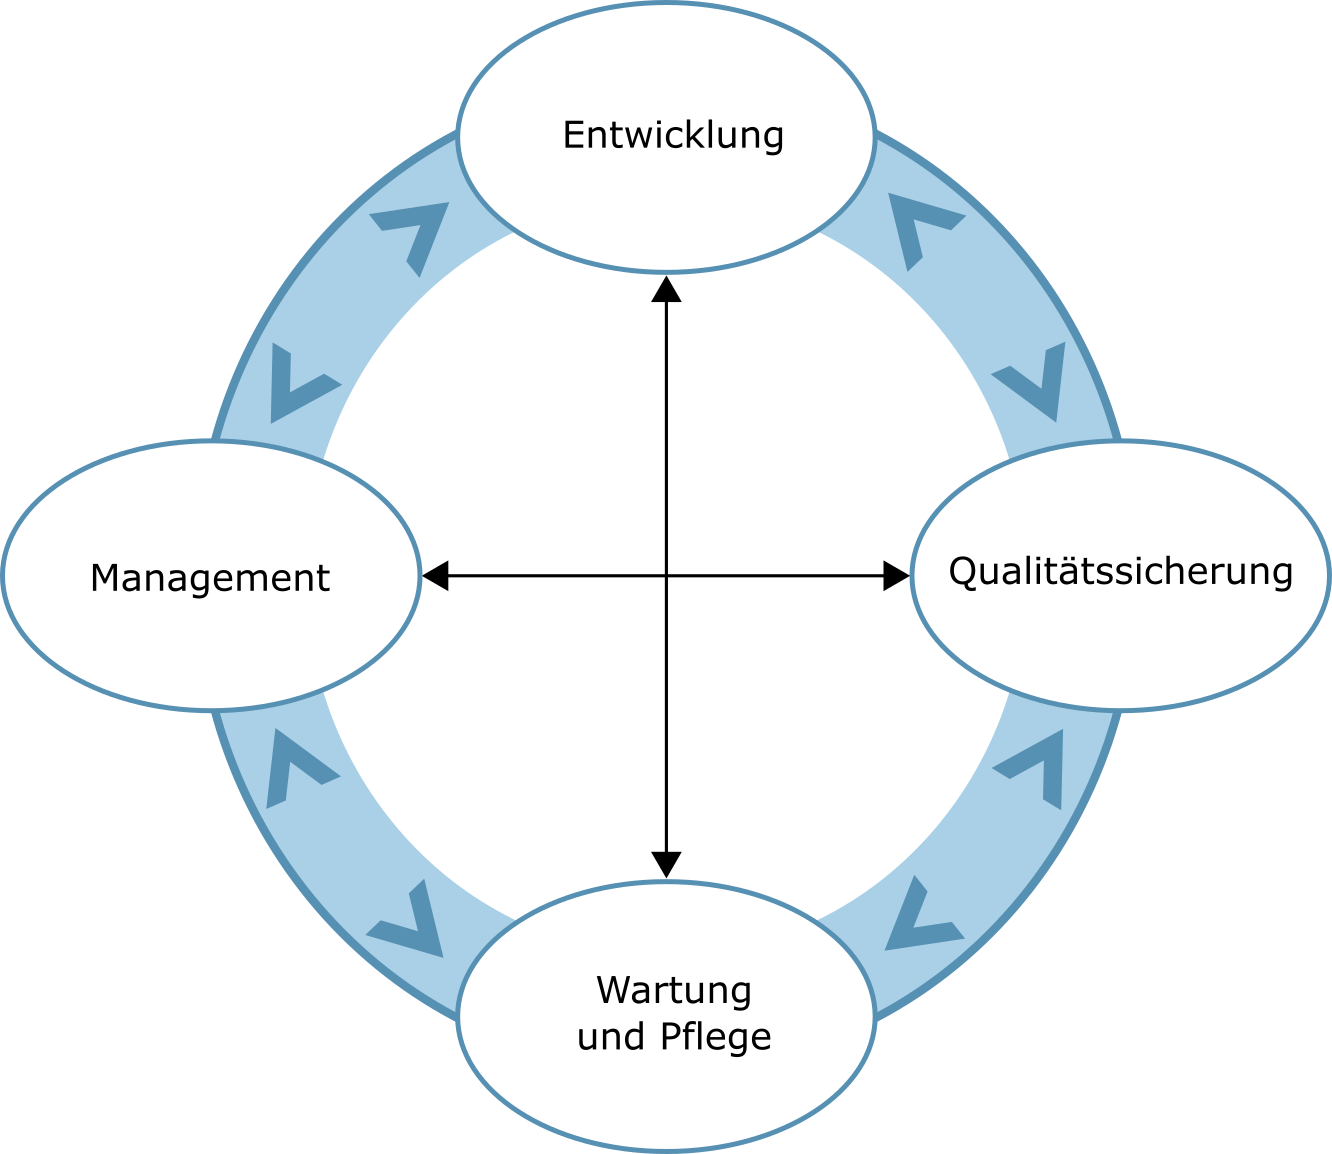
\includegraphics[width=0.5\textwidth]{./images/AbbEntwicklgProzess.png}
  \captionsetup{name=Abb.,font=footnotesize}
  \caption{Phasen im Software-Entwicklungsprozess (zyklischer Ansatz)}
\end{figure}
\newpage


\textbf{Entwicklung}
\newline
Die Software-Entwicklung hat die Aufgabe ein Produkt zu erstellen, das die geforderten Qualit"atseigenschaften besitzt. Der Entwicklungsprozess wird im Allgemeinen in eine Reihe von Aktivit"aten aufgeteilt, deren Ergebnisse einzelne Teilprodukte sind. Solche Aktivit"aten werden nach zeitlichen, begrifflichen, technischen und/oder organisatorischen Kriterien zu Phasen zusammengefasst.
\smallbreak
\textbf{Management}
\newline
Das Software-Management ist erforderlich, um den Entwicklungsprozess zu \textbf{planen}, zu \textbf{organisieren}, zu \textbf{leiten} und zu \textbf{kontrollieren}. Entwicklung und Management im Software-Entwicklungsprozess sind vielfach voneinander abh"angig. Die Einf"uhrung neuer Methoden und Tools kann zu Ver"anderungen in den organisatorischen Strukturen f"uhren.
\smallbreak
\textbf{Qualit"atssicherung}
\newline
Die Sicherstellung einer geforderten Softwarequalit"at muss durch eine entwicklungsbegleitende Software-Qualit"atssicherung erreicht werden. Dazu sind eine Reihe von konstruktiven und analytischen Ma"snahmen durchzuf"uhren. Die Ma"snahmen der Qualit"atssicherung werden dabei sowohl von der Entwicklung (die verwendeten Methoden, Tools und Programmiersprachen erfordern bestimmte Sicherungs- und Pr"ufma"snahmen), als auch vom Management durch organisatorische Zuordnung der Qualit"atssicherung zum Entwicklungsprozess beeinflusst.
\smallbreak
\textbf{Wartung und Pflege}
\newline
Nachdem ein Softwareprodukt zur Anwendung freigegeben wurde, beginnt die Wartung und Pflege, d. h. es gilt alle nach Inbetriebnahme auftretenden Fehler zu beseitigen, das Anwendungssystem an ver"anderte Bedingungen anzupassen und es bei Vorliegen neuer Anforderungen weiterzuentwickeln. Art und Umfang der Wartungst"atigkeiten sind auch von der Gew"ahrleistung der Qualit"atssicherung abh"angig, d. h. eine schlechte Produktqualit"at f"uhrt zwangsl"aufig zu h"aufigeren Fehleranteilen.

%-------------------------------------------------------------------------------
% Phasen der Entwicklung (wasserfallartig)
%-------------------------------------------------------------------------------
\newpage
\begin{figure}[H]
  \centering
  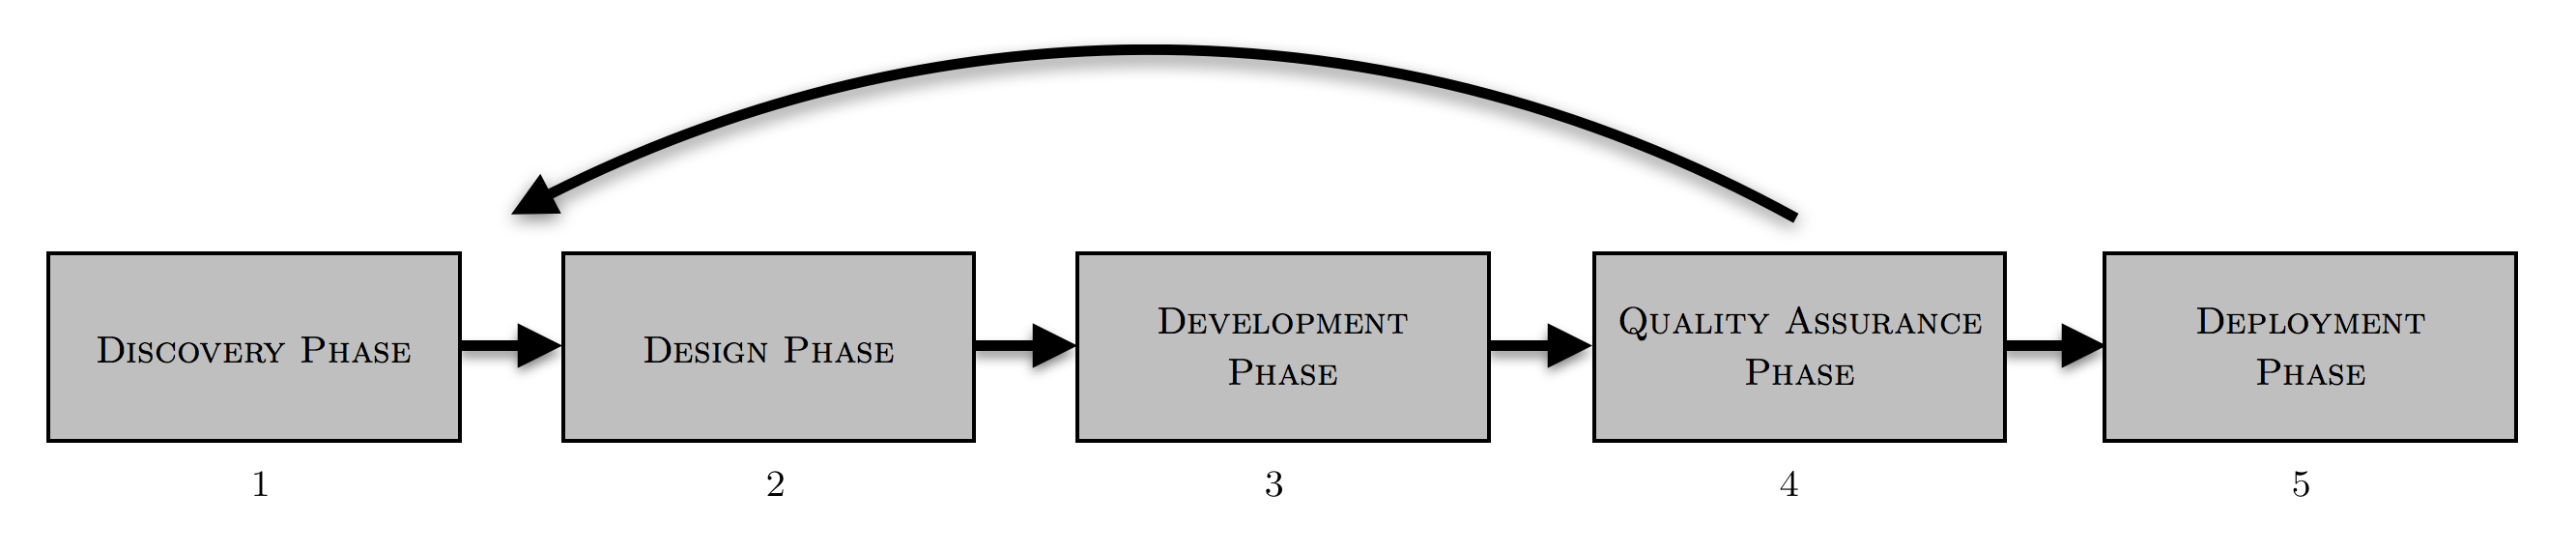
\includegraphics[width=1\textwidth]{./images/Softwarezyklus.png}
  \captionsetup{name=Abb.,font=footnotesize}
  \caption{Phasen im Software-Entwicklungsprozess (wasserfallartiger Ansatz)}
\end{figure}

\underline{\textbf{1. Discovery Phase:}}
\smallbreak
Diese Phase beinhaltet laut Balzert(1998)\supercite{Balzert1998} die \textbf{Analyse-} und \textbf{Definitionsphase}.
In der \textbf{Analysephase} wird die Ausgangssituation beschrieben,
die Ziele definiert und der daraus resultierende Ressourcenaufwand (\enquote{Scope of Work}) eruiert.\smallbreak
Diese Phase l"asst sich in folgende Aktivit"aten unterteilen:
\begin{itemize}
\item in eine Voruntersuchung (Marktanalyse, Trends, Kundenanfragen - \enquote{Idea Dump}),
\item eine Erhebung der Ist-Situation,
\item eine Erstellung einer "Ubersicht der Bestandteile (\enquote{Information Architecture}),
\item eine Durchf"uhrbarkeitsuntersuchung (\enquote{Proof of Concept})
\end{itemize}
Diese m"unden in einem Projektplan und einer aus der Wirtschaftlichkeitsbetrachtung ergebenden Projektkalkulation.
\smallbreak
In der \textbf{Definitionsphase} werden die Anforderungen an das geplante Softwaresystem aus Anwendersicht und Pr"amissen f"ur die Realisierung des Softwaresystems definiert.\smallbreak
Diese Phase l"asst sich in folgende Aktivit"aten unterteilen:
\begin{itemize}
\item Ermittlung der Anforderungen
\item Beschreibung und Festlegung der Anforderungen
\item Validierung der Anforderung auf Konsistenz, Vollst"andigkeit und technische Durchf"uhrbarkeit
\end{itemize}

Diese Aktivit"aten resultieren in einem Daten- bzw. Funktionsmodell samt Benutzerschnittstelle und Projektplan und der sich darausergebenden Produktdefinition.

\bigbreak
\underline{\textbf{2. Design Phase:}}
\smallbreak
Diese Phase beinhaltet laut Balzert(1998)\supercite{Balzert1998} die \textbf{Entwurfsphase}.

In der \textbf{Entwurfsphase} wird ein softwaretechnischer Entwurf erarbeitet und beinhaltet folgende Aktivit"aten:
\begin{itemize}
  \item Analyse der Einsatzbedingungen sowie der Umgebungs- und Randbedingungen
  \item Definition der Systemkomponenten
  \item Entwurf der Systemarchitektur (Komponenten, deren Zusammenwirken und Anordnung)
  \item Entwurf der Schnittstellen und Festlegen ihrer Wechselwirkungen
  \item Validierung der Systemarchitektur
\end{itemize}
Sie m"undet in einer Beschreibung der Struktur des Software-Entwurfs und der Systemkomponenten.

\bigbreak
\underline{\textbf{3. Development Phase:}}
\smallbreak
Diese Phase beinhaltet laut Balzert(1998)\supercite{Balzert1998} die \textbf{Implementierungsphase}.

In der \textbf{Implementierungsphase} wird die Umsetzung der Entwurfsergebnisse in eine ausf"uhrbare Form "uberf"uhrt und eine Sicherung der Richtigkeit und Fehlerfreiheit der Ergebnisse der Systemimplementierung gew"ahrleistet.

Sie beinhaltet folgende Aktivit"aten:
\begin{itemize}
  \item Verfeinerung der Algorithmen f"ur die einzelnen Systemkomponenten
  \item Kodierung / Generierung der Algorithmen
  \item "Uberf"uhrung des logischen Datenmodells in ein physisches DB-Konzept
  \item Pr"ufung der semantischen Richtigkeit der Systemkomponenten
  \item Test der Syntax und gegebenenfalls Korrektur der fehlerhaften Systemkomponenten
  \item Pr"ufung des Zusammenwirkens der Systemkomponenten unter realen Bedingungen
  \item Feststellen und Beseitigen der Fehler im Softwaresystem
\end{itemize}
Sie m"undet in einer Bereitstellung der Quelltexte f"ur die Systemkomponenten, der Protokolle der Komponententests und Systemtests und generierten Datenobjekten und Datenstrukturen.
\bigbreak
\underline{\textbf{4. Quality-Assurance Phase:}}
\smallbreak
Diese Phase beinhaltet laut Balzert(1998)\supercite{Balzert1998} die \textbf{Abnahme-/ Einf"uhrungsphase}.

In der \textbf{Abnahme-/ Einf"uhrungsphase} Abnahme des fertiggestellten Softwareproduktes und Einf"uhrung beim Anwender realisiert.

Sie beinhaltet folgende Aktivit"aten:

\begin{itemize}
  \item "Ubergabe des Softwareproduktes einschlie"sslich Dokumentation an den Auftraggeber
  \item Durchf"uhrung eines Abnahmetests
  \item Installation des Softwareproduktes in dessen Zielumgebung
  \item Schulungen der sp"ateren Benutzer der Software
  \item Inbetriebnahme des Produktes
\end{itemize}

Sie m"undet im Erfolgsfall in ein gut dokumentiertes "ubergebenes Softwareprodukt.
\bigbreak
\underline{\textbf{5. Deployment Phase:}}
\smallbreak

Diese Phase beinhaltet laut Balzert(1998)\supercite{Balzert1998} die \textbf{Wartungs-} und \textbf{Pflegephase}.

In dieser Phase beinhaltet die Gew"ahrleistung der produktiven Nutzung des Anwendungssystems, Fehlerbeseitigung am Softwaresystem in der Betriebs- bzw. Nutzungsphase und die Realisierung notwendiger "Anderungs- und Erarbeitungsarbeiten.

Sie beinhaltet folgende Aktivit"aten:
\begin{itemize}
  \item Wartung: Stabilisierung und Optimierung der Produktinstallation
  \item Pflege: Anpassungen und Erweiterungen
\end{itemize}

Sie endet mit der Auslieferung und der Wartung der Software und resultiertert in einer maximalen Kundenzufriedenheit.
\begin{figure}[H]
  \centering
  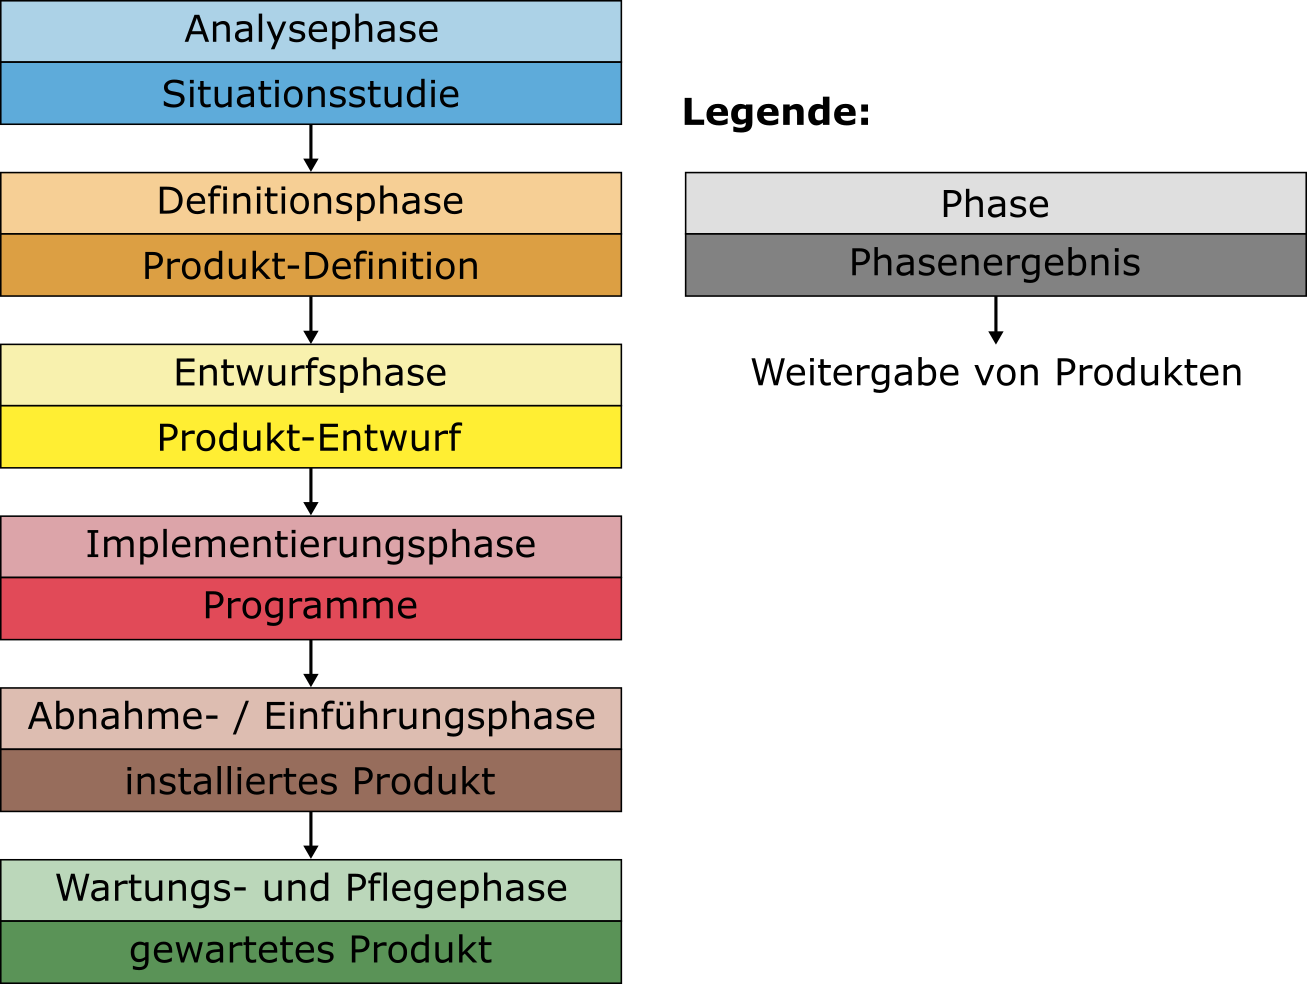
\includegraphics[width=0.8\textwidth]{./images/AbbPhaseneinteilung.png}
  \captionsetup{name=Abb.,font=footnotesize}
  \caption{Phaseneinteilung (wasserfallartig) nach Balzert(1998)\supercite{Balzert1998}}
\end{figure}


%-------------------------------------------------------------------------------
% #3
%-------------------------------------------------------------------------------
\newpage
\subsection{"Ubung SWT-03}
\subsubsection*{Aufgabe:}

\begin{framed}
\textbf{Prinzipien}
\smallbreak
Geben Sie bitte zu jedem Prinzip der Softwaretechnik (Abstraktion, Strukturierung, Hierarchisierung, Modularisierung, Standardisierung) ein Beispiel an. Wo ist Ihnen das schon begegnet und wo k"onnte das in der Softwaretechnik angewendet oder wirksam werden?
\bigbreak
\small Bearbeitungszeit: 10 Minuten
\end{framed}
\bigbreak
\bigbreak
\subsubsection*{L"osung:}
\textbf{Abstraktion}
- Beispiel: Modellbildung - User (Authentifizierung)
\smallbreak
Angenommen es gibt in einer Applikation verschiedene Sichtweisen.
Zum Beispiel eine normale User-Sicht welche in ihren Rechten beschr"ankt ist und sich daraus eingeschr"ankte Nutzungsm"oglichkeiten ergeben.
Gerade bei der Entwicklung einer ACL (Access-Control-List) bzw. einer rollenbasierten Authentifizierung innerhalb einer Applikation benutzt man Abstraktionen um nicht alle Rechte/Rollen und deren Konsequenzen bis ins Detail zu konkretisieren, sondern ein abstraktes Modell der Rechte zu entwickeln.
Man spricht dabei zum Beispiel von einem Benutzer-Kontext und einen Administrativen-Kontext.

In Bezugnahme zu sogenannten CRUD-Anwendungen sind in dem Benutzer-Kontext nur lesende Zugriffe auf das Inhaltsmodell m"oglich , wohingegen in dem Administrativen-Kontext ein Vollzugriff m"oglich ist.

Der Komplexit"atsgrad steigt mit dem Funktionsumfang, wenn man zum Beispiel dem User erlaubt eigene CRUD-Inhalte in vollem Umfang zu verwalten - so muss das Inhaltsmodel an das Usermodel gebunden werden.
Um die Komplexit"at in diesem Fall einzugrenzen bedient man sich zum Beispiel der klassenbildenden Abstraktion. Man abstrahiert den Sachverhalt auf die gemeinsamen Merkmale (im obigen Beispiel das R - Read) und bildet spezielle Merkmale (C - Create , U - Update und D - Delete).

Im obigen Beispiel wird die Inhaltsmenge die man aus dem Benutzer-Kontext konsumieren kann als Teilmenge der aus dem Administrativen-Kontext gegebenen Inhaltsmenge angesehen.
Man konkretisiert diese Inhaltsmenge nicht sondern abstrahiert nur deren Authentifizierung darauf. Durch Abstraktion ist es m"oglich das komplexe Problem Authentifizierung auf verschiedene Ebenen zu verteilen. Diese Trennung wird durch das Erfassen des Wesentlichen und das Weglassen von Besonderem realisiert.

\newpage

\textbf{Strukturierung}
- Beispiel: Architektur einer Webapplikation (MVC Pattern)

Das Prinzip der Strukturierung kann man am Beispiel des Architektur Patterns MVC sehr gut erkl"aren.
Es strukturiert eine Applikation durch die Trennung des Inhalts (Business Logik - Controller) vom Design (das Frontend - View).

Der Vorteil liegt in der unabh"angigen Entwicklung des Frontends vom Entwicklungsstand der Applikation. Es erm"oglicht somit eine parallele Entwicklung von Front- und Backend. Das Prinzip hat eine gro"se Bedeutung f"ur den Entwicklungsprozess einer Applikation.
% Es hat den Vorteil das Frontend unabh"angig (parallel) vom Entwicklungsstand der Applikation entwickelt werden kann - das Prinzip hat eine grosse Bedeutung f"ur den Entwicklungsprozess einer Applikation.

Mithilfe von Development-Seeds (f"ur die Entwicklung k"unstlich erstellte Datenbest"ande) ist es dem Frontend Entwickler m"oglich abgetrennt von der Business Logik zu entwickeln - es stellt somit eine elementare Basis f"ur die Arbeitsteilung dar.

Dar"uberhinaus hilft es bei der Bew"altigung der Komplexit"at und f"uhrt zu einer erh"ohten Verst"andlichkeit f"ur Produkt und Prozess.

Durch Abtrennung dieser Dom"anen erh"oht es zudem die Wartbarkeit und die Einarbeitung in ein fremdes Softwareprodukt (Reverse-Engineering).

Als Beispiel k"onnte man den klassischen Entwicklungsprozess einer Webapplikation anf"uhren. Es wird unabh"angig vom Controller die View entwickelt.
Die View (Frontend) kann auch erst einmal mit hardcodierten Inhalten entwickelt werden und sp"ater mittels Templating mit produktiven Daten gef"ullt werden.

Oft kommen die produktiven Daten aus diversen Subsystemen (Backend) die f"ur einzelne Entwickler nicht allumfassend "uberschaubar sind.
Das Frontend muss sich also bei guter Gesamtstrukturierung nicht um die Richtigkeit/Validit"at der Daten k"ummern und kann sich voll und ganz auf die Entwicklung der View's konzentrieren.

Ein weiteres Beispiel f"ur Strukturierung ist das Prinzip der ``Partials'' in einem Applikationsfrontend. Durch Partials ist es m"oglich ein Problem nur einmal zu definieren/auszuprogrammieren und entspricht dem DRY (``Don't repeat Yourself'') Best-Practise der Softwaretechnik.

\textbf{Hierarchisierung}
- Beispiel: Partial-Hierarchie

Das Prinzip der Hierarchisierung ist ein Spezialfall der Strukturisierung und bezeichnet eine Rangordung.

Als Beispiel kann man das Prinzip der Partials noch einmal aufgreifen. Dort wird eine Struktur der Applikation ausgehend von einem Main/Layout-Partial hierrarchisch realisiert.
Die Applikation wird in Sektionen strukturiert. Es werden also bestimmte Sektionen in den Code injeziert (``Yielding'').

Es ist also m"oglich eine Applikation in Hauptseiten und Unterseiten bzgl. der Hierarchie zu strukturieren.
Das Prinzip der Hierarchie liegt einer Baumstruktur zu grunde. (Das Main/Layout-Partial stellt in diesem Fall die Wurzel dar.)

\newpage
\textbf{Modularisierung}
- Beispiel: Packagemanager in Programmiersprachen

In jedem "Okosystem einer Programmiersprache hat man M"oglichkeiten auf Module/Pakete zur"uckzugreifen und bestimmte Probleme nicht noch einmal l"osen zu m"ussen. (diverse Packagemanager: npm - node.js, gems - ruby, composer - php, maven - java, pip - python , cmake - c))

Ein Modul/Paket bietet die M"oglichkeit der Aufgliederung eines Softwaresystems in diverse Subsysteme. Das hat den Vorteil das die Komplexit"at durch das Prinzip ``divide and conquer'' geb"andigt wird.
Diese Module bieten diverse Schnittstellen f"ur den In/Output und sind in sich abgeschlossen und wiederverwendbar.

Dar"uberhinaus sind Module in sich wartbar (vom Maintainer) und abgekapselt vom Hauptsystem. Der Nachteil sind die entstehenden Abh"angigkeiten - Dependencies.

Ich hatte zum Beispiel in Java das Problem der Serialization/Deserialization von JSON.
Nat"urlich h"atte ich auch das Rad neu erfinden k"onnen und es mit den Werkzeugen der Programmiersprache selbst l"osen k"onnen. (Aus einem String einen JSON bauen k"onnen.)
Viel einfacher ging das aber "uber ein Modul/Paket von Google GSON, welches eine Abstraktionsebene dazwischen geschalten hat und letztlich schneller zum zur Probleml"osung f"uhrte.

Ein weiteres Beispiel w"are die Authentifizierung gegen"uber eines Domaincontrollers "uber das LDAP-Protokoll.
Hierbei habe ich auf ein Composer-Package ADLAP2 zur"uckgegriffen, welches die Authentifizierung gegen einen Domaincontroller erm"oeglichte.
Dabei musste ich nicht die genaue Funktionsweise verstehen, sondern lediglich die Anwendung des Modules "uber ihre Schnittstellen.

Als Anlaufstelle f"ur Packages/Module in diversen Sprachen nutze ich "uberwiegend Github - weil dort 99\% aller meiner Probleme in einer Form schon gel"ost wurden und ich sie auf die jeweilige Anforderung meines Systems abstrahieren kann.

Es geht mittlerweile soweit, dass ich an diversen Stellen Contribute (Code beitrage) da ich Nutzungsanforderungen entdecke die vom Modul/Package noch nicht abgedeckt werden.

Problematisch sehe ich jedoch das durch die Nutzung von Fremdmodulen Abh"angigkeiten zu dem jeweiligen Package/Modul entstehen k"onnen und die Gefahr besteht das es aufgrund der Abh"angigkeit Probleme gibt bei einem Major-Update des Hauptsystems.

Dar"uberhinaus sehe ich es als problematisch an, gerade bei sensiblen Mechanismen e.g. Authentifizierung einer Applikation, nicht nur auf die Funktionalit"at eines Moduls/Packages zu vertrauen, sondern viel mehr auf die Kompetenz der Entwickler in Bezug auf die Sicherheit eines Softwaresystems.

Dem gegen"uber steht die Open-Source Bewegung wo jeder Code-Review betreiben kann und die Software so qualitativ hochwertiger ist in Bezug auf deren Sicherheit.

(Ein Paper zu der Problematik: https://arxiv.org/pdf/1704.02786.pdf)


\newpage
\textbf{Standardisierung}
- Beispiel: betriebsinterne Konventionen in der Arbeit mit GIT

Das Prinzip der Standardisierung beinhaltet die Vereinheitlichung des Entwicklungsprozesses und des Produktes. Der wichtigste Aspekt ist die Kostenminifizierung. Der Aufwand wird gemindert durch das Einf"uhren von Standards.
Es entwickelte sich dazu das Paradigma ``Convention over Configuration'', was die Konvention vor die Konfiguration stellt und so den Konfigurationsaufwand mindert. (e.g. Ruby on Rails)

Dies beginnt mit einer schematischen Dokumentation (Dokumentationsvorlage),
der Verwendung von Standards zur grafischen Modellbeschreibung (UML),
der Verwendung bew"ahrter Design- (Design-Pattern) und Implementierungs-Muster
bis hin zu einer Kodierung, die strikt vereinbarte Regel (Code Convention) einh"alt.

Beispielhaft einige betriebsinterne Konventionen f"ur Git:
\begin{itemize}
  \item Namensgebung der Fix Branches / Feature Branches (Issue \# + description)
  \item Vorlagen f"ur Commit-Messages
  \item Vor einem Merge-Request alle Commits in einem Commit zusammenzufassen  (``commit squashing - has the benefit of keeping your git history tidy'')

\end{itemize}


%-------------------------------------------------------------------------------
% #4
%-------------------------------------------------------------------------------
\newpage
\subsection{"Ubung SWT-04}
\subsubsection*{Aufgabe:}

\begin{framed}
\textbf{Recherche}
\smallbreak
Recherchieren Sie bitte im Internet "uber Softwaretechnik oder Softwareengineering. Welche Bereiche interessieren Sie ganz besonders?
\bigbreak
\small Bearbeitungszeit: 30 Minuten
\end{framed}
\bigbreak
\bigbreak
\subsubsection*{L"osung:}

Die Softwaretechnik gliedert sich in mehrere spannende Teilbereiche.

Mich pers"onlich intressiert besonders das Build-Management. Das automatisierte ``Bauen'' (und ``Testen'') einer Software im Hinblick auf eine reibungslose kontinuierliche Auslieferung (Continous Integration/Delivery) einer Software.

Softwaresysteme sind meines Erachtens immer lebende Projekte, die nie wirklich abgeschlossen sind und sich inkrementell stets verbessern oder eine neue Anwendung als ``Dependency'' in einem anderen Softwaresystem finden (oder geforked und abgewandelt werden).
Aus dieser lebendigen Eigendynamik ergeben sich immer neue Abh"angigkeiten/Anforderungen/Herausforderungen an das Projekt.

Dar"uber hinaus interessiert mich vor allem die Vertiefung der Arbeit mit einem Versions Control System, insbesondere mit Git.
Ein Verst"andnis f"ur einen Git-Flow zu entwickeln. Wie man zum Beispiel das Einfliessen von neuem Code (Contributions) organisiert.

Sehr spannend fande ich in diesem Zusammenhang auch das Einhalten einer Konvention zur Versionierung (Semantic-Versioning) um der ``Dependency Hell'' Einhalt zu gebieten.

Zus"atzlich bin ich st"andig an der Optimierung der Deployment-Pipeline interessiert.
Als zentraler Bestandteil der ``Continous Delivery'' wird dabei st"andig neuer Code released. Dieser Vorgang(build , test, deploy) sollte automatisiert ablaufen.

Ansonsten interessiert mich auch das Anforderungsmanagement um ein Gef"uhl zu entwickeln den Umfang/Scope eines Softwareprojektes besser absch"atzen zu k"onnen.

Einen Weitblick zu entwickeln um effektiver und zielgerichteter arbeiten zu k"onnen und das Projekt in die richtige Richtung zu leiten.

%-------------------------------------------------------------------------------
% #5
%-------------------------------------------------------------------------------
\newpage
\subsection{"Ubung SWT-05}
\subsubsection*{Aufgabe:}

\begin{framed}
\textbf{Wissensfragen zur Lerneinheit}
\smallbreak
Versuchen Sie die Fragen schriftlich zu beantworten ohne noch einmal in der Lerneinheit nachzuschlagen.
\begin{enumerate}
\item An welche Best Practices erinnern Sie sich oder welche haben Sie verinnerlicht?
\item Warum ist es sinnvoll Softwarefehler fr"uh zu erkennen?
\item Was geht in Softwareprojekten typischerweise schief?
\item Kennen Sie (Standardisierungs-)Organisationen, die sich mit Software besch"aftigen?
\end{enumerate}
\bigbreak
\small Bearbeitungszeit: 15 Minuten
\end{framed}
\bigbreak
\bigbreak
\subsubsection*{L"osung:}
\begin{enumerate}
\item Best-Practise:
\smallbreak
\textbf{DRY} (Don't repeat yourself)

Ich habe besonders verinnerlicht Probleme nur an einer Stelle zu l"osen und die L"osung universell zug"anglich zu machen und mich nicht zu wiederholen. Sollte einmal die Probleml"osung erweitert oder ge"andert werden so gibt es nur eine Stelle im Code wo das erledigt/gefixed werden muss.
Ich bin stets daran interessiert bestimmte Vorg"ange zu automatisieren. Das vermindert die Fehleranf"alligkeit und ist produktiver.

\textbf{KISS} (Keep it short and simple)

Dieses Best-Practise beinhaltet den Ansatz Probleme/Anforderungen einfach und zielorientiert zu l"osen. Ein gutes Pferd springt nur so hoch wie es muss um auch die n"achste H"urde noch nehmen zu k"onnen.
Bei der Entwicklung ist es immer ein Dreieck aus Zeit,Geld und Qualit"at. Nat"urlich erwartet man ein qualitativ hochwertiges Ergebnis was in Abh"angigkeit von der investierten Zeit und Geld steht.
Die Dinge zu simplifizieren mindert den Zeitanspruch und man hat mehr Zeit qualitativ hochwertiger zu entwickeln.

Auch bei der Problemdefinition ist das KISS-Prinzip sehr wichtig um die Dinge auf den Punkt zu bringen. Zum Beispiel das Abstrahieren einer Problemstellung durch Weglassen von unwesentlichen Elementen. (s.a. \textbf{``25 Words or less''})
\newpage
\textbf{No Bang} (divide and conquer)

Es ist einfacher die gro"se und komplexe Problemstellung in kleinere Probleme zu unterteilen. Der Code wird sauber strukturiert und ist dadurch universell anwendbarer. Das hilft bei der Entwicklung einer ``Knowledge Repository'', weil man viele kleine L"osungen (``Snippets'')hat, an denen man sich bei der L"osung weiterer Probleme in anderen Projekten bedienen kann.

\textbf{Vorgehensmodell}

In Bezug auf die Methodik einer Softwareentwicklung ist es eine Best-Practise ein entsprechendes Vorgehensmodell zu haben. Wenn die Anforderungen nicht klar und in sich abgeschlossen sind, bietet sich eher ein agiles als ein wasserfallartiges Vorgehensmodell an.
Oftmals k"onnen die Stakeholder eine Anforderung nicht klar und abgeschlossen ausformulieren und es hat sich f"ur mich als Best-Practise erwiesen erst einmal etwas anzubieten und dann in Revision mit den Stakeholdern inkrementell sich den daraus ergebenene Anforderungen anzun"ahern. (agil)

\textbf{Workflow}

Bevor man entwickelt ist es f"ur mich wichtig einen guten Workflow zu haben. Eine Dev-Environment einzurichten die einen effizienten Workflow erm"oglicht und der sp"ateren Prod-Environment entspricht um den Aufwand f"ur das Deployment zu minimieren.


\item Warum ist es sinnvoll Softwarefehler fr"uh zu erkennen?
\smallbreak

In einem komplexen Softwaresystem ist es wichtig Fehler fr"uhzeitig zu erkennen weil sich Abh"angigkeiten auf diesen Fehler entwickeln k"onnen und sich daraus Folgefehler entwickeln. Man sollte die Robustheit einer Probleml"osung stets im Blick haben um die Probleml"osung universell anwendbarerer zu machen. Dabei ist es wichtig die Edge-Cases zu definieren und zu testen. (TDD)
\begin{figure}[H]
  \centering
  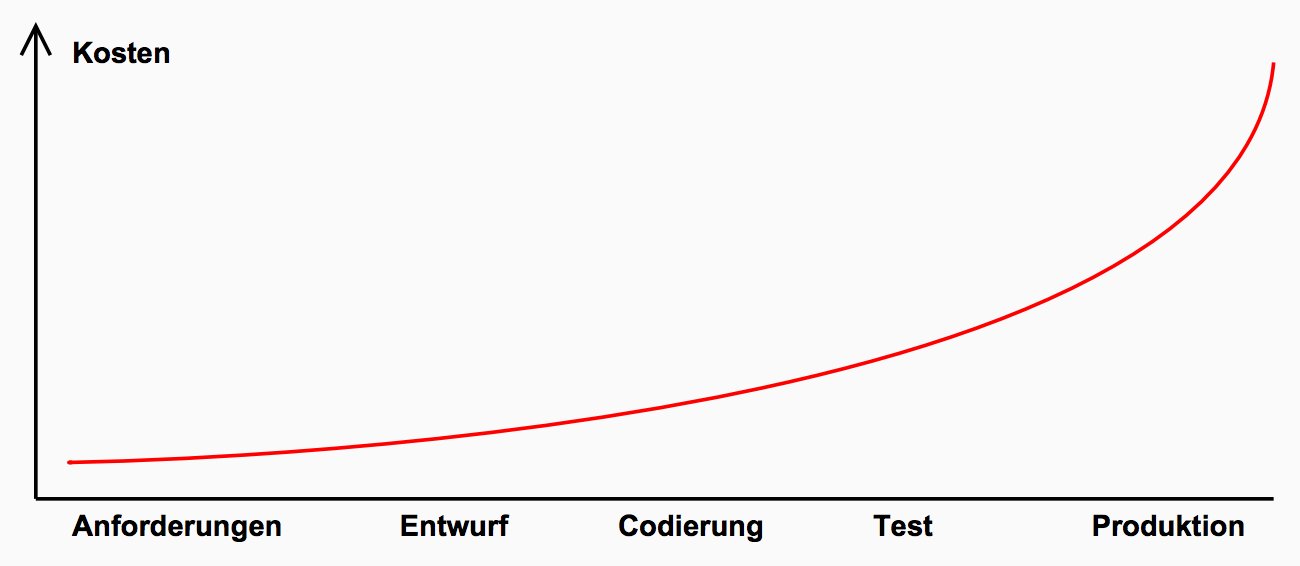
\includegraphics[width=0.8\textwidth]{./images/Aenderungskosten.png}
  \captionsetup{name=Abb.,font=footnotesize}
  \caption{"Anderungskosten in der Softwareentwicklung}
\end{figure}
% \begin{center}
% 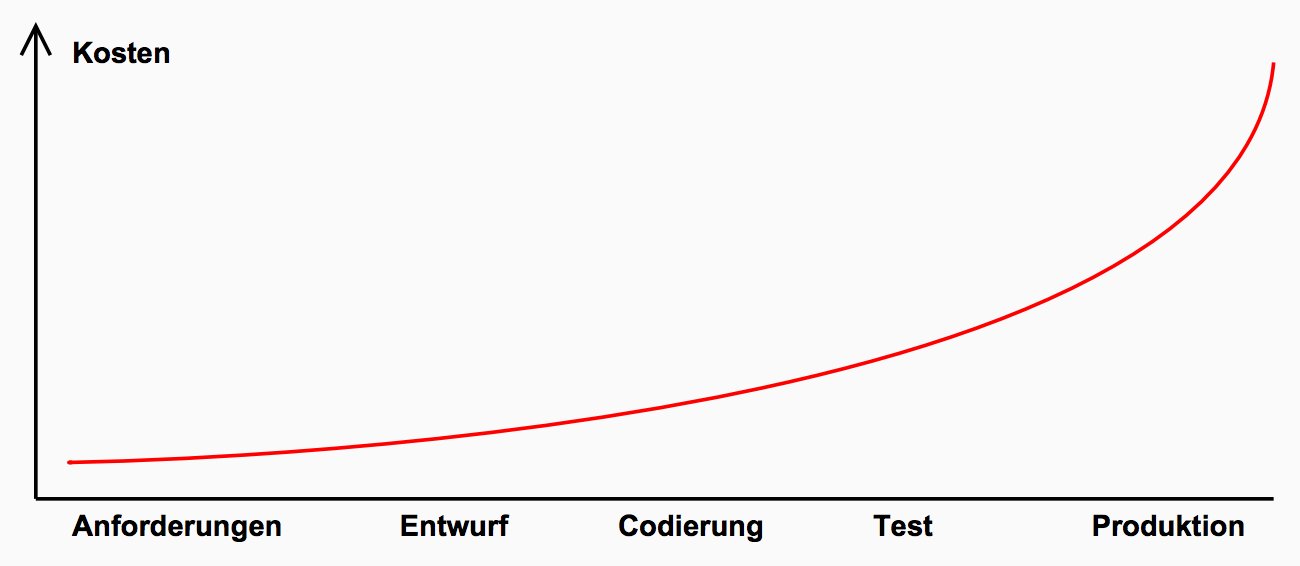
\includegraphics[width=0.9\textwidth]{./images/Aenderungskosten.png}
% \end{center}

\newpage
\item Was geht in Softwareprojekten typischerweise schief?

\begin{itemize}
\item unrealistische oder unausgesprochene Projektziele
\item falsche Sch"atzung ben"otigter Ressourcen
\item schlecht definierte Requirements
\item schlechte Berichte "uber Projektfortschritt
\item nicht gemanagte Risiken
\item schlechte Kommunikation zwischen Kunden, Entwicklern und Benutzern
\item Verwendung unausgereifter Technologie
\item Unf"ahigkeit, die Projektkomplexit"at in den Griff zu kriegen
\item nachl"assige Entwicklungspraktiken
\item schlechtes Projektmanagement
\item ``politische'' Gr"unde der Beteiligten
\item kommerzieller Druck
\end{itemize}


\item Kennen Sie (Standardisierungs-)Organisationen, die sich mit Software besch"aftigen?


\begin{itemize}
  \item Object Management Group (OMG) -> UML
  \item Organization for the Advancement of Structured Information Standards (OASIS)
  \item Deutsches Insitut f"ur Normung (DIN)
  \item World Wide Web Consortium (W3C) -> XML, HTML
  \item ECMAScript - Javascript -> e.g. Node.js ,V8 (google chrome)
  \item Institute of Electrical and Electronics Engineers (IEEE)
  \item American Standard Code for Information Interchange (ASCII)
  \item American National Standard Institute (ANSI)
  \item Department of Defense (DoD)
  \item Association of Computing Machinary (ACM)
  \item European Committee for Standardization (DEN)
  \item Gesellschaft f"ur Informatik e.V. (GI)
\end{itemize}
\end{enumerate}

%-------------------------------------------------------------------------------
% #6
%-------------------------------------------------------------------------------
\newpage
\subsection{"Ubung SWT-06}
\subsubsection*{Aufgabe:}

\begin{framed}
\textbf{Fehlerquellen}
\smallbreak
H"aufige Fehlerq"ullen in Softwareprojekten sind:
\bigbreak
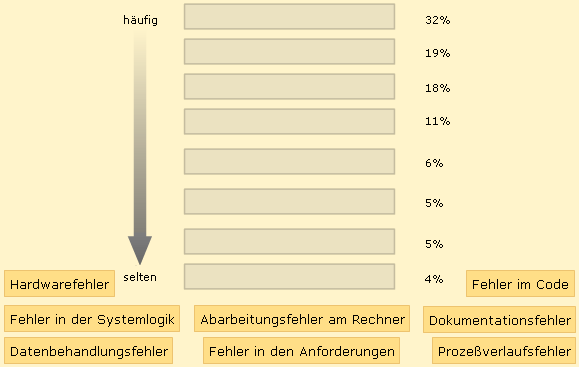
\includegraphics[width=1.0\textwidth]{./images/ueb01-06.png}
\end{framed}
\bigbreak
\bigbreak
\subsubsection*{L"osung:}

\begin{enumerate}
  \item Fehler in der Systemlogik 32\%
  \item Dokumentationsfehler 19\%
  \item Abarbeitungsfehler am Rechner 18\%
  \item Fehler im Code 11\%
  \item Datenbehandlungsfehler 6\%
  \item Fehler in den Anforderungen 5\%
  \item Proze"sverlaufsfehler 5\%
  \item Hardwarefehler 4\%
\end{enumerate}

%-------------------------------------------------------------------------------
% #7
%-------------------------------------------------------------------------------
\newpage
\subsection{"Ubung SWT-07}
\subsubsection*{Aufgabe:}

\begin{framed}
\textbf{Phaseneinteilung}
\smallbreak
Ordnen Sie die Phasen und Ergebnisse des Softwarelebenszyklus in der richtigen Reihenfolge an.
\bigbreak
\begin{center}
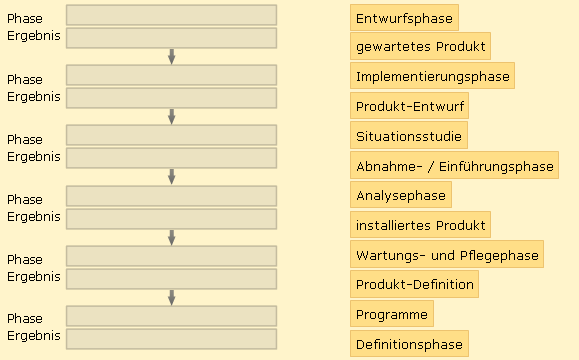
\includegraphics[width=0.9\textwidth]{./images/ueb01-07.png}
\end{center}
\end{framed}
\bigbreak
\bigbreak
\subsubsection*{L"osung:}
\begin{enumerate}
  \item Analysephase -> Situationsstudie
  \item Definitionsphase -> Produkt-Definition
  \item Entwurfsphase -> Produkt-Entwurf
  \item Fehler im Code -> Fehler im Code
  \item Implementierungsphase -> Programme
  \item Abnahme-/ Einf"uhrungsphase -> installiertes Produkt
  \item Wartungs- und Pflegephase -> gewartetes Produkt
\end{enumerate}









%-------------------------------------------------------------------------------
% Literatur - Glossar - Akronyme
%-------------------------------------------------------------------------------

\clearpage
\setlength\bibitemsep{10pt}
\printbibliography[heading=bibintoc]
\newpage
\printglossary[type=main,title=Glossar]
\printglossary[type=\acronymtype, title=Akronyme]


%-------------------------------------------------------------------------------
% ENDE
%-------------------------------------------------------------------------------

\end{document}
